% Created 2024-09-10 Tue 20:54
% Intended LaTeX compiler: xelatex
\documentclass[11pt]{article}
\usepackage{graphicx}
\usepackage{longtable}
\usepackage{wrapfig}
\usepackage{rotating}
\usepackage[normalem]{ulem}
\usepackage{capt-of}
\usepackage{hyperref}
\usepackage{minted}
\usepackage[a4paper, margin=2.5cm]{geometry}
\usepackage{minted}
\usepackage{fontspec}
\setmonofont{Iosevka}
\setminted{fontsize=\small, frame=single, breaklines=true}
\usemintedstyle{emacs}
\usepackage[backend=biber,style=apa]{biblatex}
\addbibresource{citation.bib}
\usepackage{amsmath}
\allowdisplaybreaks
\author{Baley Eccles - 652137}
\date{\textit{{[}2024-09-04 Wed 12:39]}}
\title{ENG231 - Electrical Machines And Transformers - Assignment 1}
\hypersetup{
 pdfauthor={Baley Eccles - 652137},
 pdftitle={ENG231 - Electrical Machines And Transformers - Assignment 1},
 pdfkeywords={},
 pdfsubject={},
 pdfcreator={Emacs 29.4 (Org mode 9.8)}, 
 pdflang={English}}
\begin{document}

\maketitle
\tableofcontents

\section{ENG231 - Electrical Machines And Transformers - Assignment 1}
\label{sec:orgee24842}
\subsection{Question 1}
\label{sec:orgeed3db3}
\begin{itemize}
\item 1: Alternatting current in the primary coil
\begin{itemize}
\item When an alternating current flows throug the primary coil, it creates a time varing magnetic field. Which is described by Ampere's Law, which states that an electric current produces a magnetic field.
\end{itemize}
\item 2: Magnetic flux generation
\begin{itemize}
\item The time varing magnetic field creates a magnetic flux in the transformer. From Faraday's Law, the induced EMF in a coil is proportional to the the rate of change of magnetic flux in the coil \(\left( \mathcal{E}\propto \frac{\partial \Phi}{\partial t}\right)\).
\end{itemize}
\item 3: Induction in the secondary coil
\begin{itemize}
\item The magnetic flux generated in the primary coil links to the secondary coil and produces an EMF dependent on the number of turns in the secondary winding. As described by Farday's Law \(\left( \mathcal{E}=-N\frac{\partial \Phi}{\partial t}  \right)\)
\end{itemize}
\item 4: Transfer of power
\begin{itemize}
\item In an ideal transformer the power induced in the secondary winding is equal to the power supplied to the primary winding. That is \(P_1=P_2\) or \(V_1I_1=V_2I_2\), where \(V\) is the voltage and \(I\) is the current.
\end{itemize}
\end{itemize}
\subsection{Question 2}
\label{sec:org6f479bb}
\begin{align*}
P_{in}&=P_{out} \\
P_{out}&=V_{in}I_{in} \\
P_{out}&=240\cdot 1.14 \\
P_{out}&=273.6W
\end{align*}
\subsection{Question 3}
\label{sec:org3deec9a}
Two possible power losses in the transformer are, resistive losses due to the copper not having zero resistance and eddy currents in the core.
To reduce the power losses due to eddy currents in the core, we can laminate the core.By spliting the core into seperate thin sheets of the cores material. This will reduce the power losses by making it harder for eddy currents to form.
\subsection{Question 4}
\label{sec:org82a0762}
\subsubsection{a}
\label{sec:org45aeab8}
\begin{minted}[]{octave}
clear
clc
pkg load symbolic
I_rms=1.14;
I_peak=I_rms*sqrt(2);
f=50;
w=2*pi*f;
t=0:0.00001:0.1;
i=I_peak*sin(w*t);
clf;
plot(t,i);
titleStr = sprintf('Current plot of the Arlec 2166');
title(titleStr, 'FontSize', 10);
xlabel('Time (s)');
ylabel('Current (A)');
filename = sprintf('ENG231-1.png');
print(filename,'-dpng','-r100');
\end{minted}


\begin{center}
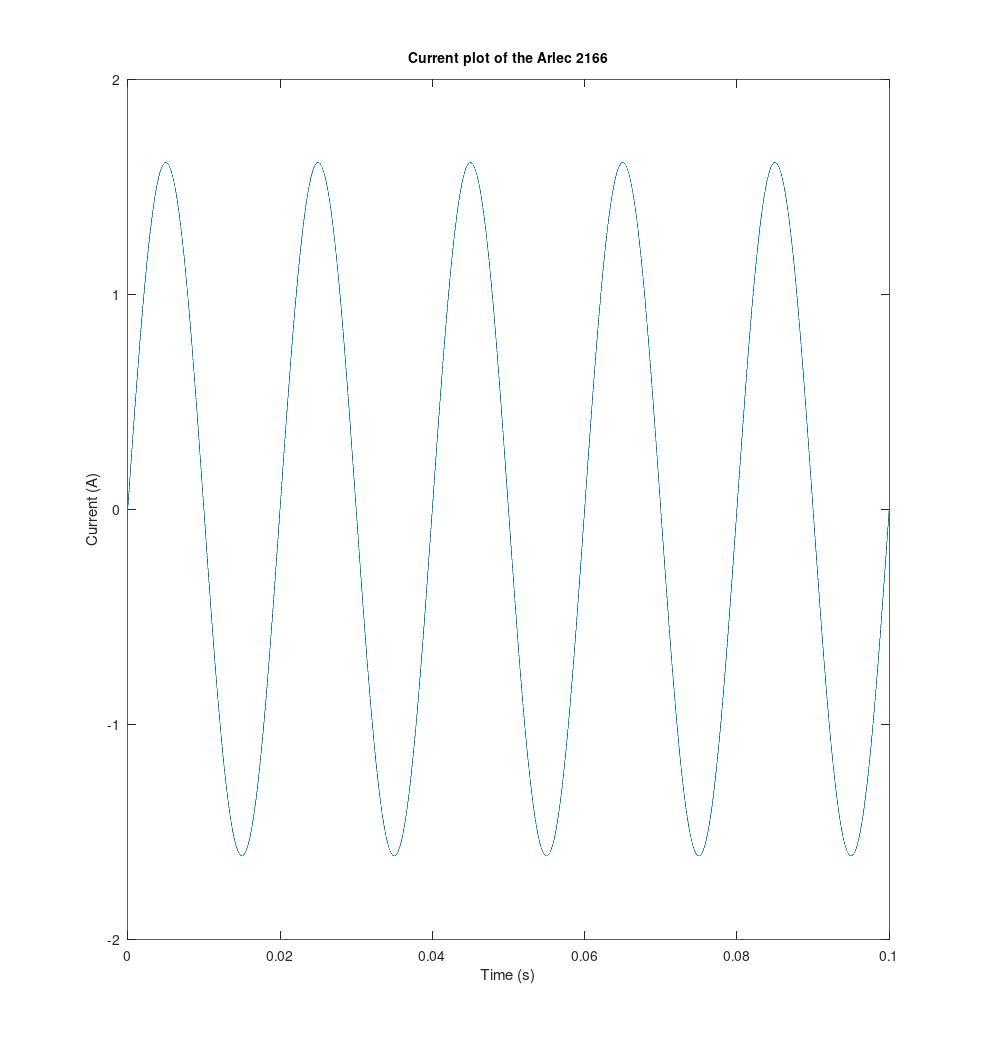
\includegraphics[width=.9\linewidth]{ENG231-1.png}
\end{center}
\subsubsection{b}
\label{sec:org3ae25fe}
\begin{minted}[]{octave}
M_sat=1.4*10^6;
h_0=2230;
M=M_sat*(2/pi)*atan(6*i/5);
H=h_0*i;
u_0=4*pi*10^(-7);
B=u_0*(M+H);

clf;
hold on;
plot(i, M, 'b', 'DisplayName', 'Magnetization Curve');
linear = (i >= -0.5) & (i <= 0.5); % Example range for linearity
plot(i(linear), M(linear), 'r', 'LineWidth', 2, 'DisplayName', 'Linear Region');
titleStr = sprintf('Plot of the hysteresis of the Arlec 2166');
title(titleStr, 'FontSize', 10);
xlabel('Current (A)');
ylabel('Magnetic Flux Density (T)');
legend show;
hold off;
filename = sprintf('ENG231-2.png');
print(filename,'-dpng','-r100');
\end{minted}


\begin{center}
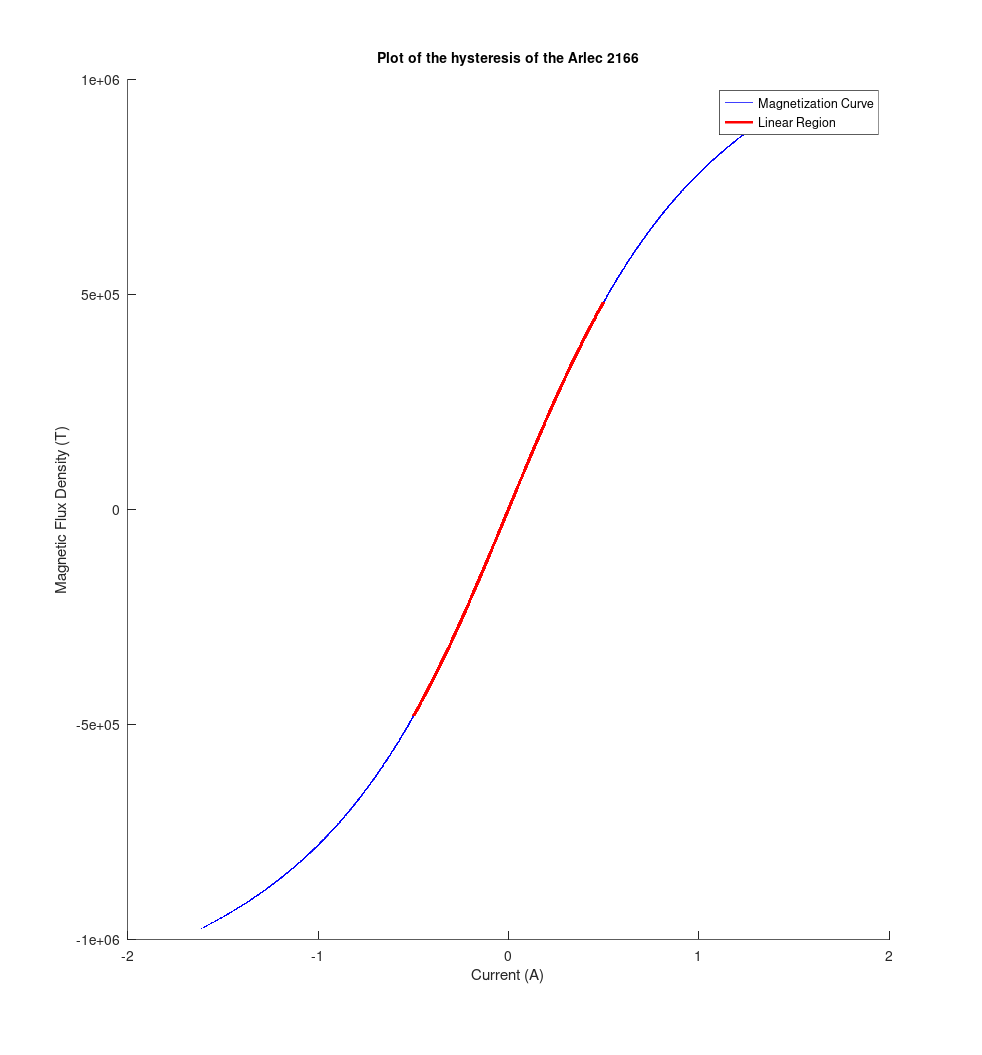
\includegraphics[width=.9\linewidth]{ENG231-2.png}
\end{center}
\subsubsection{c}
\label{sec:orgbefebdc}
\begin{minted}[]{octave}
M_sat=1.4*10^6;
h_0=2230;
M=M_sat*(2/pi)*atan(6*i/5);
H=h_0*i;
x=M/H;
fprintf('The maximum value of the magnetic susceptibility of the core of the transformer is %f\n',max(x));
\end{minted}

The maximum value of the magnetic susceptibility of the core of the transformer is 301.847007
\subsection{Question 5}
\label{sec:org350a159}
\subsubsection{a}
\label{sec:org343b0f0}
\begin{minted}[]{octave}
clear
clc
V_rms=240;
V_peak=V_rms*sqrt(2);
f=50;
w=2*pi*f;
t=0:0.0001:0.1;
V=V_peak*sin(w*t);
clf;
hold on;
plot(t,V,'r', 'DisplayName', 'Input Voltage (V)');
titleStr = sprintf('Voltage plot of the Arlec 2166');
title(titleStr, 'FontSize', 10);
xlabel('Time (s)');
ylabel('Voltage (V)');
legend('show');
filename = sprintf('ENG231-3.png');
print(filename,'-dpng','-r100');
\end{minted}


\begin{center}
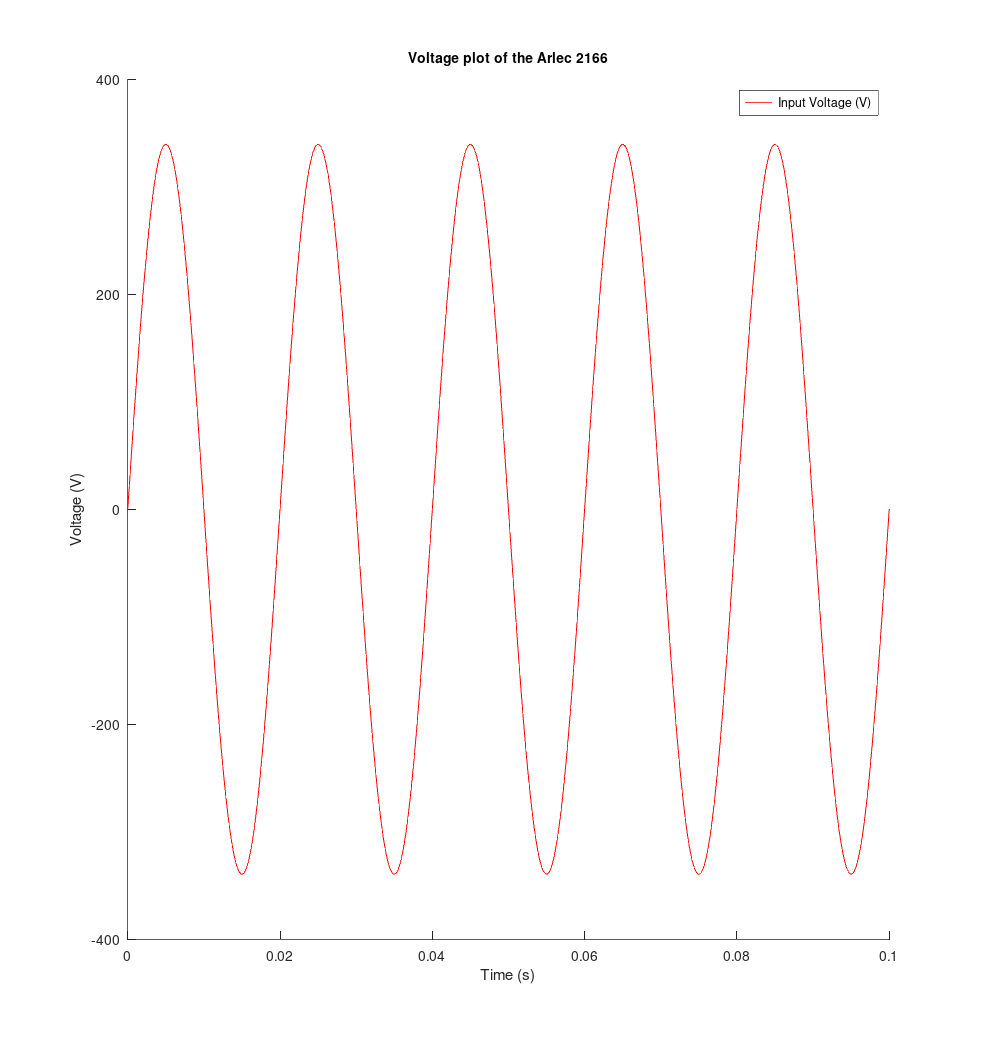
\includegraphics[width=.9\linewidth]{ENG231-3.png}
\end{center}
\subsubsection{b}
\label{sec:org3e018db}
\begin{minted}[]{octave}
clear
clc
% From Q4 Part a and b:
t=0:0.0001:0.1;
I_rms=1.14;
I_peak=I_rms*sqrt(2);
f=50;
w=2*pi*f;
i=I_peak*sin(w*t);
M_sat=1.4*10^6;
h_0=2230;

% Old code
M=M_sat*(2/pi)*atan(6*i/5);
H=h_0*i;
u_0=4*pi*10^(-7);
x_m=301.847007-1;
H=x_m*H + H;
B=u_0*H;

N=880; % From guess and check
A=3*10^(-2)*3*10^(-2);
Phi=B*A;
EMF=-N* gradient(Phi)./gradient(t);

V_rms=240;
V_peak=V_rms*sqrt(2);
f=50;
w=2*pi*f;
t=0:0.0001:0.1;
V=V_peak*cos(w*t);


clf;
hold on;
plot(t(1:end), EMF, 'b', 'DisplayName', 'Induced EMF');
plot(t(1:end), V, 'r', 'DisplayName', 'Supplied Voltage');
xlabel('Time (s)');
ylabel('Voltage (V)');
title('Induced EMF and Supply Voltage');
legend show;
E_max=max(EMF);
fprintf('The max EMF induced is %f\n', E_max);
filename = sprintf('ENG231-4.png');
print(filename,'-dpng','-r100');
\end{minted}


\begin{center}
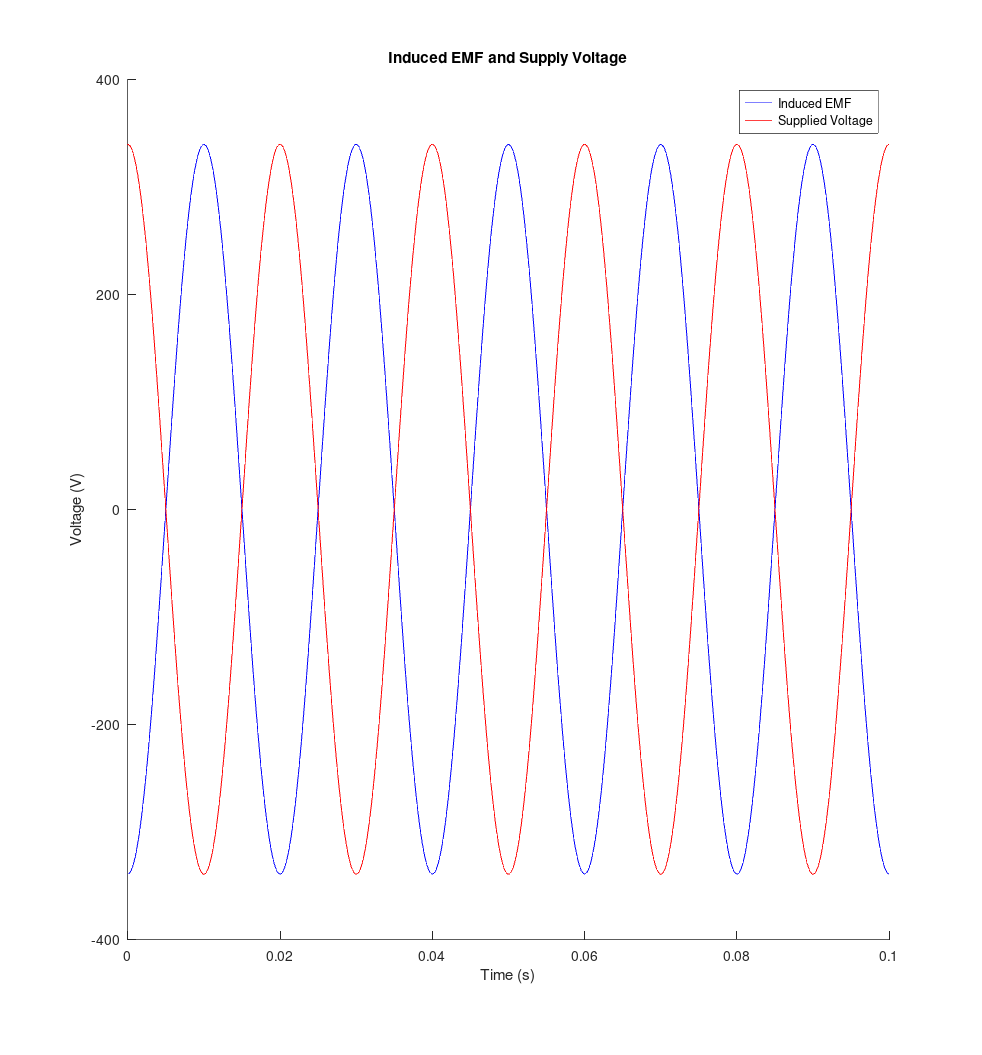
\includegraphics[width=.9\linewidth]{ENG231-4.png}
\end{center}
\subsubsection{c}
\label{sec:orgb37115f}
The induced EMF is dependent on the derivative of the flux which is dependent on the current. So the EMF will be out of phase of the current by \(90^o\).
The current lags the voltage.
\subsubsection{d}
\label{sec:org45af0fe}
It can be seen that the induced EMF is not dependent on the voltage. So, the supplied voltage and induced EMF may not be in phase with one another.
\subsubsection{e}
\label{sec:org796d35d}
\begin{minted}[]{octave}
clc
clear
A=3*10^(-2)*3*10^(-2);
t=0:0.0001:0.1;

f=50;
w=2*pi*f;
N=550;
M_sat=1.4*10^6;
h_0=2230;
u_0=4*pi*10^(-7);

I_peak1=2.5;
i1=I_peak1*sin(w*t);
H=h_0*i1;
u_0=4*pi*10^(-7);
x_m=301.847007-1;
H=x_m*H + H;
B=u_0*H;
A=3*10^(-2)*3*10^(-2);
Phi=B*A;
N=550;
E1=-N* gradient(Phi)./gradient(t);

I_peak2=0.25;
i3=10^(-1)*I_peak2*sin(3*w*t);
H=h_0*i3;
u_0=4*pi*10^(-7);
x_m=301.847007-1;
H=x_m*H + H;
B=u_0*H;
A=3*10^(-2)*3*10^(-2);
Phi=B*A;
N=550;
E3=-N* gradient(Phi)./gradient(t);

I_peak5=0.025;
i5=10^(-2)*I_peak5*sin(5*w*t);
H=h_0*i5;
u_0=4*pi*10^(-7);
x_m=301.847007-1;
H=x_m*H + H;
B=u_0*H;
A=3*10^(-2)*3*10^(-2);
Phi=B*A;
N=550;
E5=-N* gradient(Phi)./gradient(t);


ETotal=E1+E3+E5;

fprintf('The max induced EMF is %f\n',max(ETotal));


V_rms=240;
V_peak=V_rms*sqrt(2);
f=50;
w=2*pi*f;
t=0:0.0001:0.1;
V=-V_peak*cos(w*t);

clf;
hold on;
%plot(t, E1, 'b', 'DisplayName', 'Induced EMF 1');
%plot(t, E3, 'r', 'DisplayName', 'Induced EMF 2');
%plot(t, E5, 'g', 'DisplayName', 'Induced EMF 3');
plot(t, ETotal, 'DisplayName', 'Total induced EMF');
plot(t, V, 'DisplayName', 'Supply voltage');

titleStr = sprintf('Voltage');
title(titleStr, 'FontSize', 10);
xlabel('Time (s)');
ylabel('Voltage (V)');
legend('show');
hold off;
filename = sprintf('ENG231-5.png');
print(filename,'-dpng','-r100');

\end{minted}
The max induced EMF is 338.8


\begin{center}
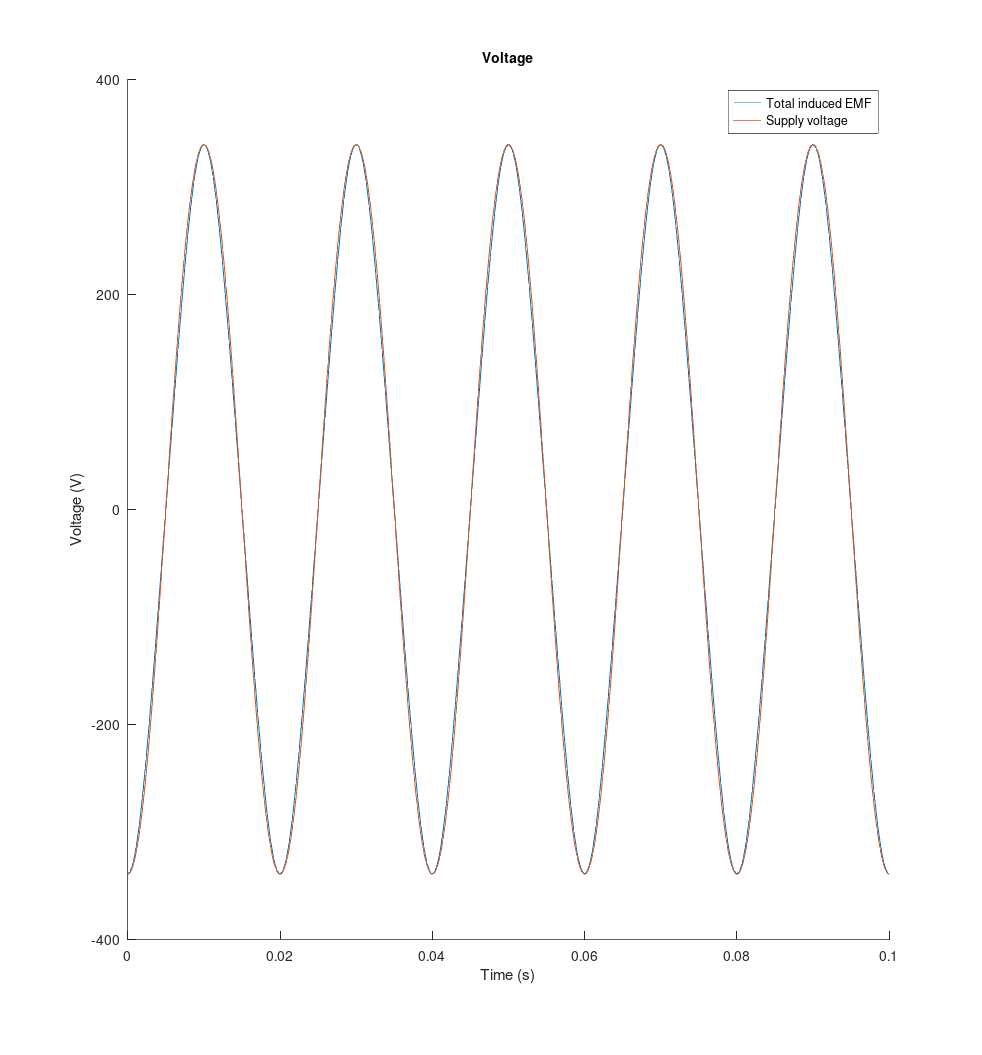
\includegraphics[width=.9\linewidth]{ENG231-5.png}
\end{center}
\subsubsection{f}
\label{sec:org13d4733}
The max induced EMF is 338.8V, so the RMS EMF is 239.6V. Which is approximately the stated RMS voltage of 240V.
\subsubsection{g}
\label{sec:orgac47323}
The number of windings is 550.
\end{document}
